\documentclass[../main.tex]{subfiles}
\graphicspath{{\subfix{../figures/}}}

\begin{document}
The first step towards finding an exceptional point and simulating the dynamics of the quantum dot system was to calculate the matrix representation of the Liouvillian. This was done numerically using an already implemented PERLind approach as well as with the Python-based QmeQ package (\cite{qmeq}) as a sanity check. The parameter space was then "scanned" for exceptional points by numerically calculating the eigenvalues of $L$ for varying $\delta\epsilon$ and $\delta\Gamma$. A degeneracy of eigenvalues was found at $\lambda_5 = \lambda_6 = \bar\lambda \approx -0.5\Gamma$, for $\delta\Gamma = 10^{-6}\Gamma$ and $\delta\epsilon \approx 0.3\Gamma$, see figure~\ref{fig:tuning}. The corresponding eigenvectors was found to also coalesce to $\ket{\rho_5}\rangle = \ket{\rho_6}\rangle = \ket{\bar \rho}\rangle$, confirming the existence of an exceptional point.
\begin{figure}[H]
    \centering
    \includegraphics[width=0.9\linewidth]{figures/tuning.png}
    \caption{hej}
    \label{fig:tuning}
\end{figure}

The full spectrum of the Liouvillian at the exceptional point is given in figure~\ref{fig:spec}. Note the existence of a zero eigenvalue ($\lambda_1$).

\begin{figure}[H]
    \centering
    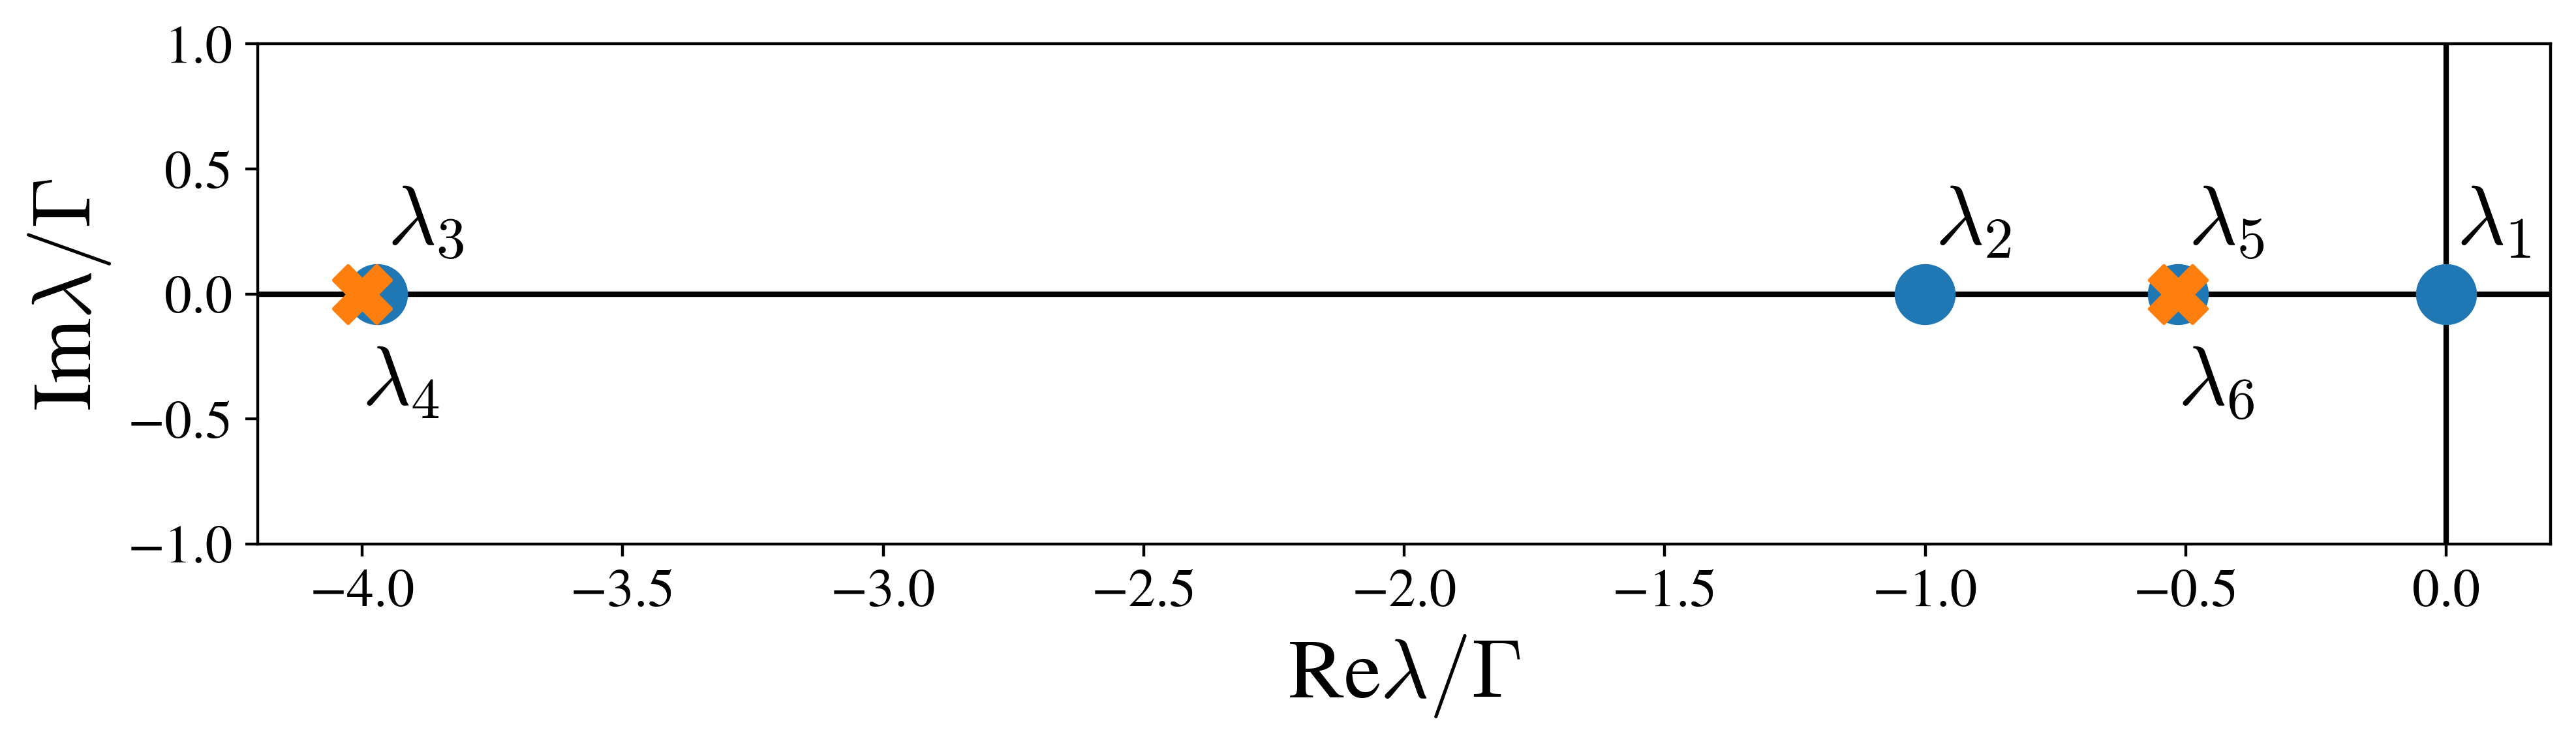
\includegraphics[width=0.8\linewidth]{figures/spectrum.png}
    \caption{hej}
    \label{fig:spec}
\end{figure}


To obtain an expression for the evolution of the system, the Lindblad equation has to be solved. In Fock-Liouville space, this is given by 
\begin{equation}
    \diff{}{t}\ket{\rho(t)}\rangle = L \ket{\rho(t)}\rangle
\end{equation}

Using equation~\eqref{eq:genmode}, the solution can be given in terms of the eigenvalues and generalized eigenvectors of $L$. Outside of an exceptional point, the Liouvillian is diagonalizable, and the terms are purely exponential. The evolution of the density operator is then given by

\begin{equation}\label{eq:dynnonep}
    \ket{\rho(t)}\rangle = \ket{\rho_{ss}}\rangle + \sum_{i=2}^6 e^{\lambda_i t} \langle\braket{\sigma_i|\rho(0)}\rangle \ket{\rho_i}\rangle
\end{equation}
where $\ket{\rho_{ss}}\rangle = \langle\braket{\sigma_1|\rho(0)}\rangle \ket{\rho_1}\rangle$ is the steady state of the system, due to the zero eigenvalue $\lambda_1=0$.

At the exceptional point, the Jordan form of $L$ and its exponential $e^{Jt}$ have to be evaluated. Since the EP is of order two, this results in a $2\times2$ Jordan block. This is the only EP, so the rest of the Jordan form is diagonal. Using equations~\eqref{eq:jordan} and~\eqref{eq:expjordan}, this results in the following Jordan form and exponential:

\begin{equation}
    J = \begin{bmatrix} 0 & 0 & 0 & 0 & 0 & 0 \\
                        0 & \lambda_2 & 0 & 0 & 0 & 0 \\
                        0 & 0 & \lambda_3 & 0 & 0 & 0 \\
                        0 & 0 & 0 & \lambda_4 & 0 & 0 \\
                        0 & 0 & 0 & 0 & \bar \lambda & 1 \\
                        0 & 0 & 0 & 0 & 0 & \bar \lambda \\ \end{bmatrix}, \; 
        e^{Jt} = \begin{bmatrix} 1 & 0 & 0 & 0 & 0 & 0 \\
            0 & e^{\lambda_2t} & 0 & 0 & 0 & 0 \\
            0 & 0 & e^{\lambda_3t} & 0 & 0 & 0 \\
            0 & 0 & 0 & e^{\lambda_4t} & 0 & 0 \\
            0 & 0 & 0 & 0 & e^{\bar \lambda t} & t \\
        0 & 0 & 0 & 0 & 0 & e^{\bar \lambda t} \\ \end{bmatrix},
\end{equation}
since $\lambda_1 = 0$.

Furthermore, the Jordan chain vector $\ket{\rho'}\rangle$ defined by $(L - \bar\lambda I)\ket{\rho'}\rangle = \ket{\bar\rho}\rangle$ and its corresponding row in $M^{-1}$, $\langle\bra{\sigma'}$, need to be calculated. Inserting this into equation~\eqref{eq:genmode}, the evolution of the density operator can be shown to be given by
\begin{equation}\label{eq:dynep}
    \begin{aligned}
        \ket{\rho(t)}\rangle = &\ket{\rho_{ss}}\rangle + \sum_{i=2}^4 e^{\lambda_i t} \langle\braket{\sigma_i|\rho(0)}\rangle \ket{\rho_i}\rangle \\ 
                               & + e^{\bar \lambda t}\left\{\langle\braket{\bar\sigma|\rho(0)}\rangle + t\langle\braket{\sigma'|\rho(0)}\rangle \right\}\ket{\bar \rho}\rangle \\ 
                               & + e^{\bar\lambda t} \langle\braket{\sigma'|\rho(0)}\rangle\ket{\rho'}\rangle.
    \end{aligned}
\end{equation}

By numerically calculating the generalized eigenvectors and the corresponding rows in $M^{-1}$, the dynamics at non-EP and at EP given by equations~\eqref{eq:dynnonep} and~\eqref{eq:dynep}, could be simulated. The results were then compared with a numerical ODE-solver, see figure X.

As discussed in the theory section, one can obtain expectation values for any relevant observable of the system from the density operator. For the parallel dot system, the main observable is the current $\hat I$, which is described in terms of the jump operator. Using equation~\eqref{eq:expec}, the current over time can be evaluated by $\braket{\hat I(t)} = \tr{(\hat \rho(t)\hat I)}$. Implementing this numerically, the current through the quantum dot system for varying parameters and initial conditions could be simulated. The first simulation involved sitting at an EP and choosing initial conditions in terms of the generalized eigenvectors, see figure~\ref{fig:diffrho0}. In figure~\ref{fig:diffde}, the dynamics of the current at and slightly away from the exceptional point was simulated.
\begin{figure}[H]
    \centering
    \begin{minipage}[t]{0.48\textwidth}
        \centering
        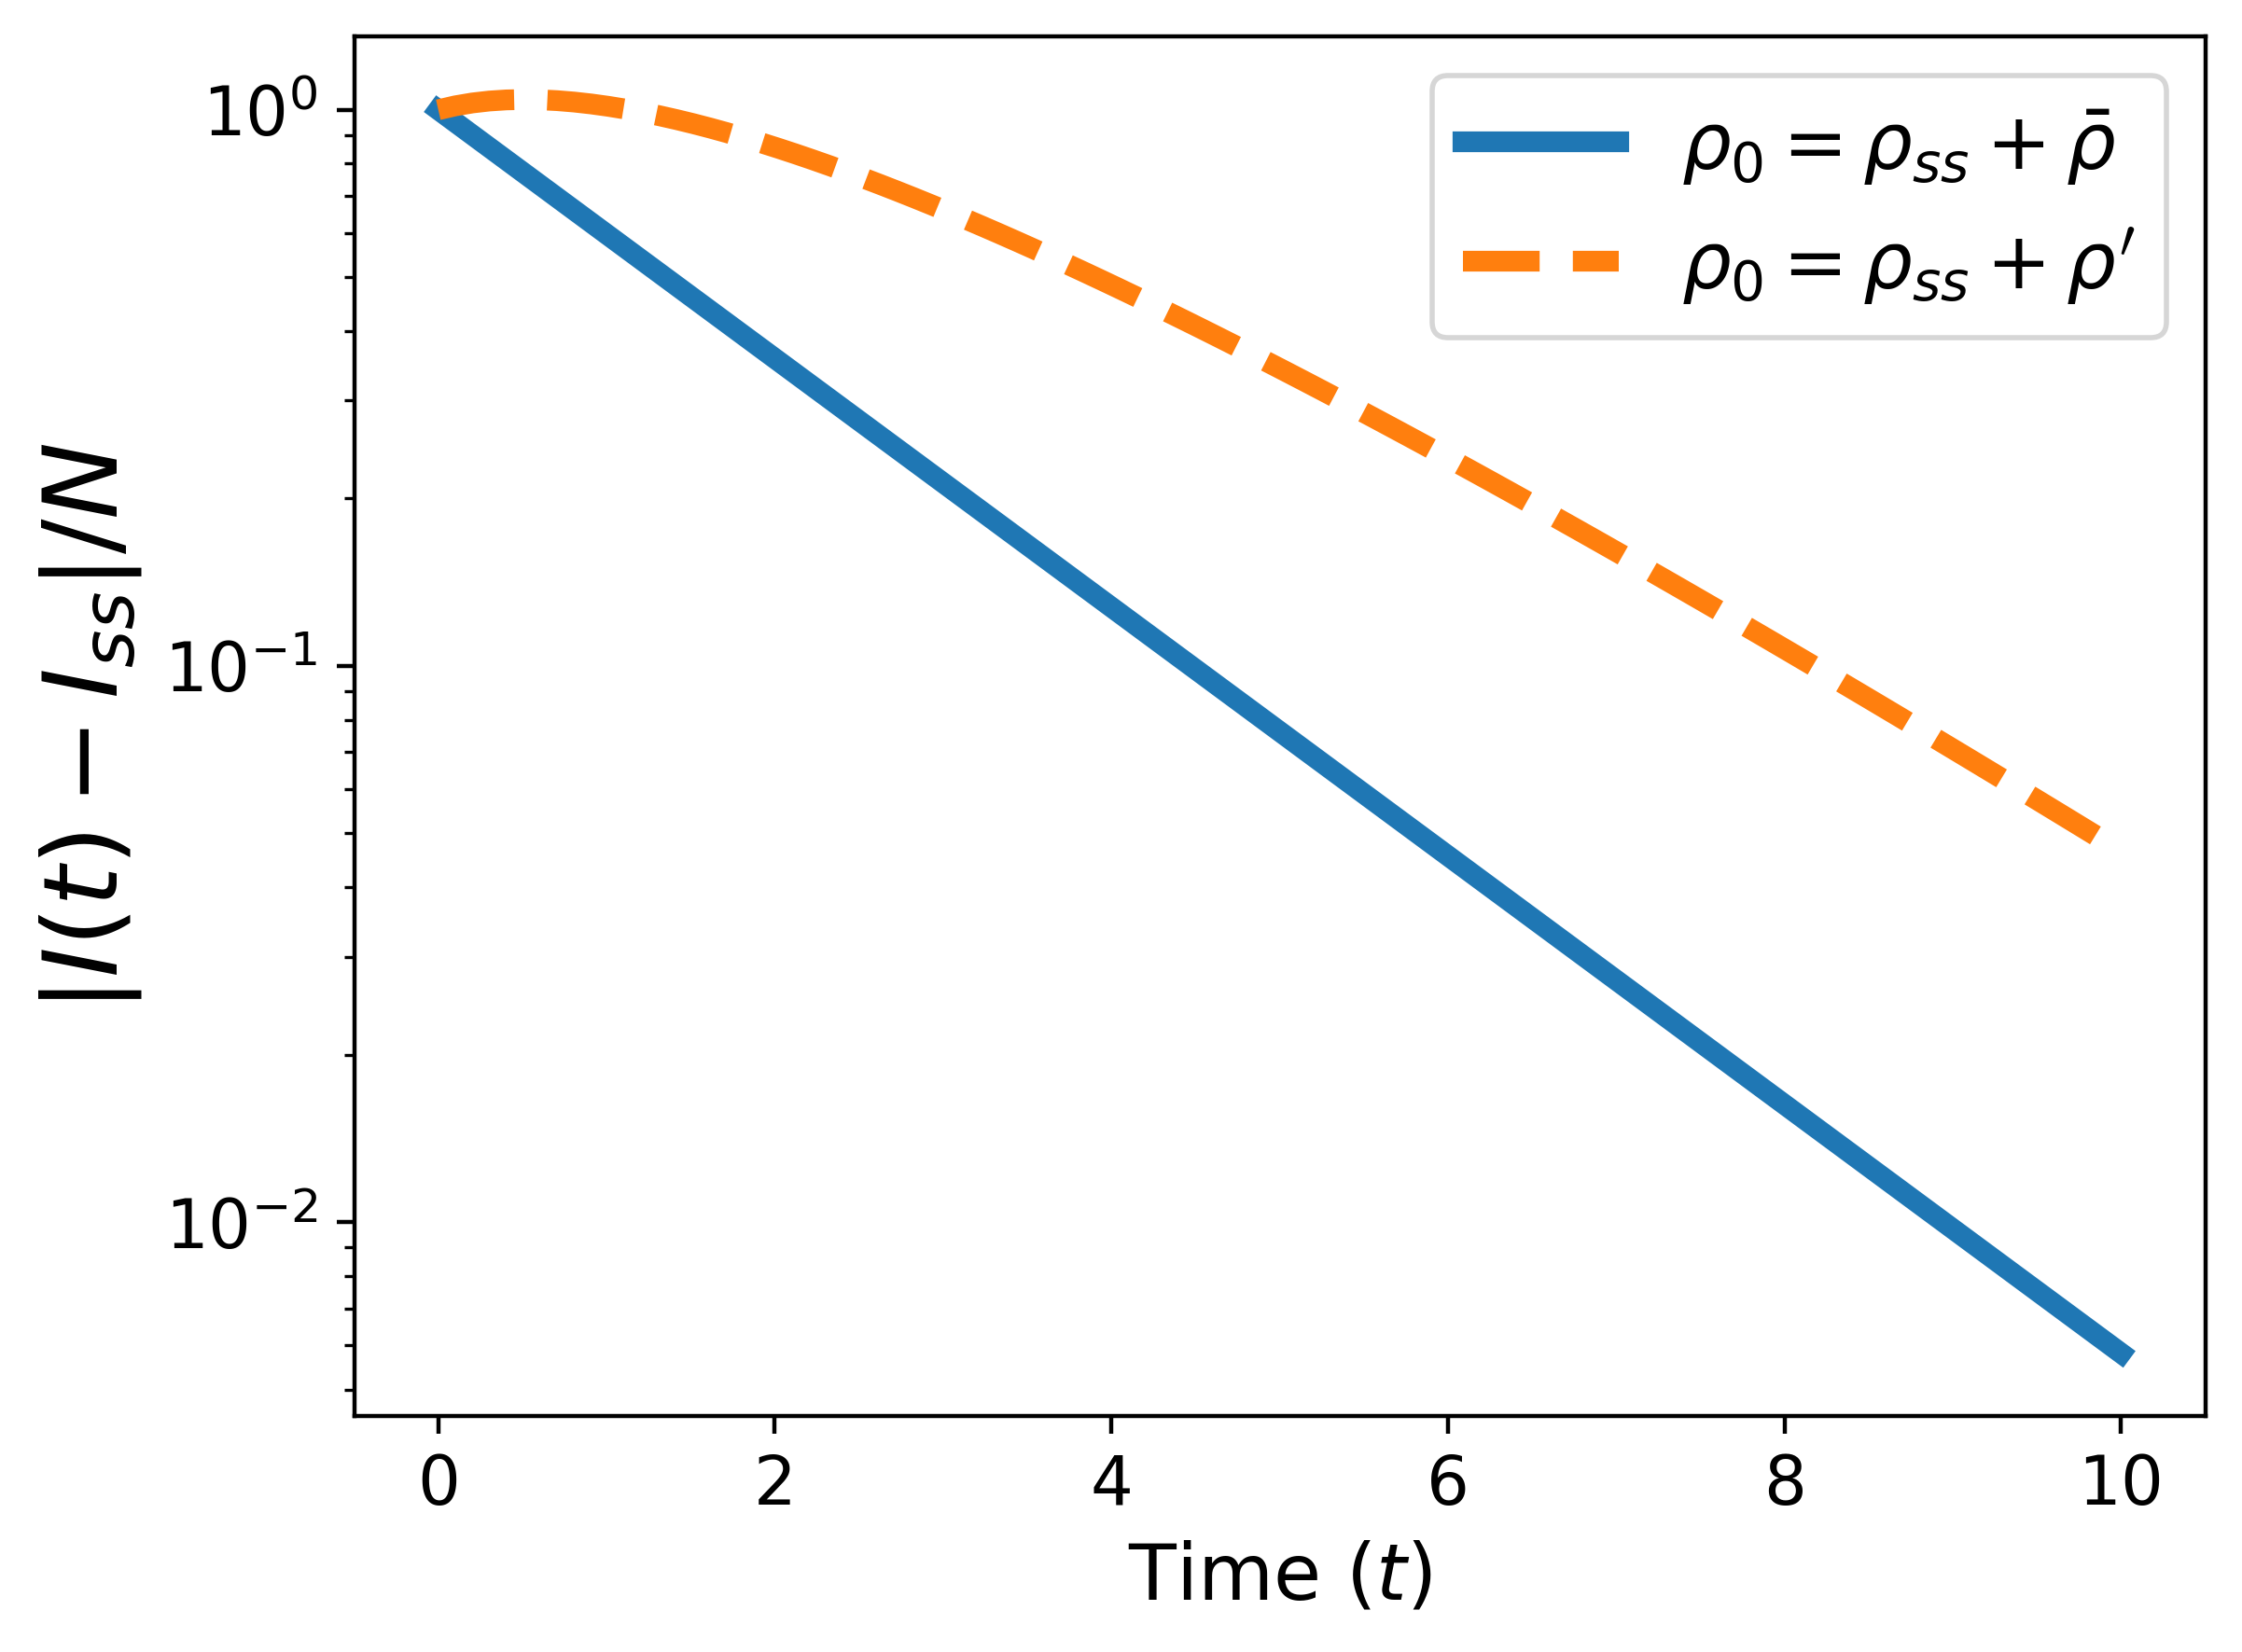
\includegraphics[width=\textwidth]{figures/current_diff_rho_0.png}
        \caption{The decay of the current towards the steady state current $I_{ss}$ in a log plot. The simulations were done at the EP with different initial conditions. A normalization by $N=|I(0) - I_{ss}|$ was done such that each curve is unity for $t=0$.}
    \label{fig:diffrho0}
    \end{minipage}\hfill
    \begin{minipage}[t]{0.48\textwidth}
        \centering
        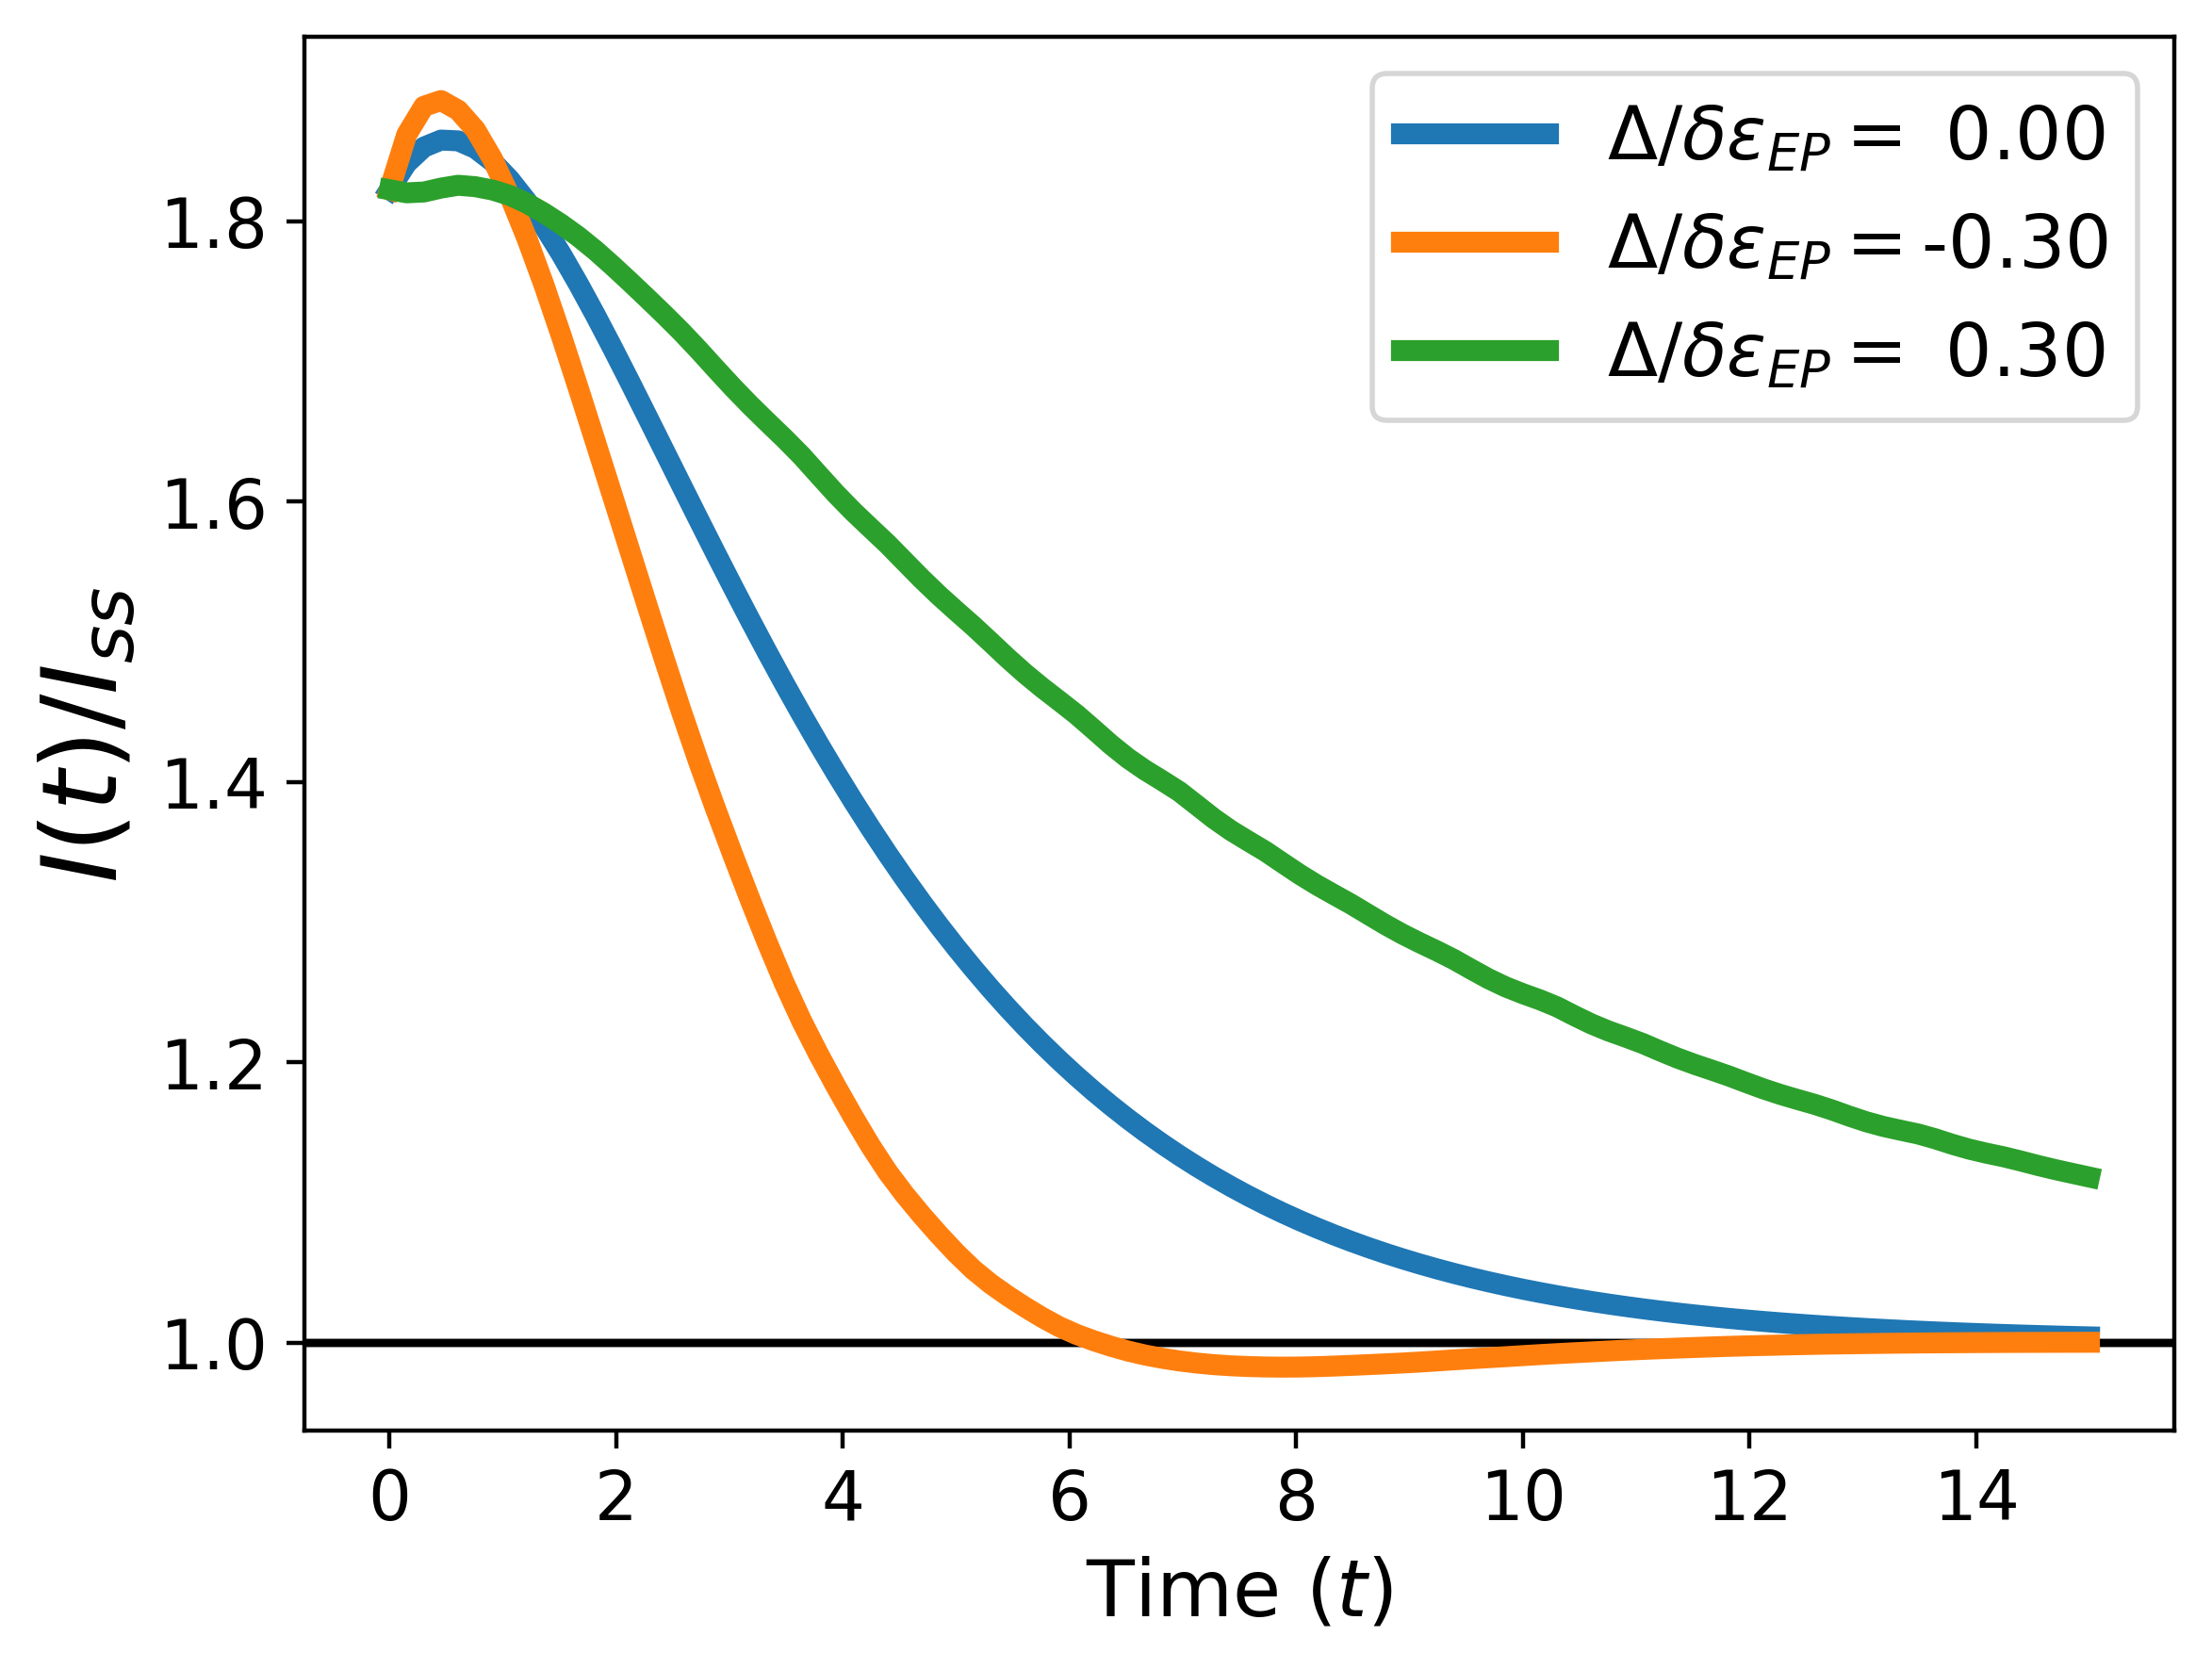
\includegraphics[width=\textwidth]{figures/curr_diff_de.png}
        \caption{The current over time for different $\delta\epsilon$, normalized by the steady state current $I_{ss}$. The solid, blue curve correspond to the system being at the EP, while the other two are slightly away from it. All simulations were done with the same initial condition.}
    \label{fig:diffde}
    \end{minipage}\hfill
\end{figure}



\end{document}
